\documentclass[class={IEEEtran}]{standalone}

\usepackage{amsmath}
\usepackage{tikz}
\usepackage{pifont}

\newcommand{\whiteding}[1]{\large{\ding{\numexpr171+#1\relax}}}

\pagestyle{empty}

\usetikzlibrary{shapes.geometric,shapes.arrows,positioning,calc,arrows.meta,math}

\tikzset{AGENT/.style={rectangle,minimum width=6.5em,minimum height=3.5ex,draw,semithick,align=flush center}}
\tikzset{ACTION/.style={rectangle,rounded corners,draw,semithick,align=flush center,fill=white}}
\tikzset{BOX/.style={draw, line width=1pt, rounded corners=5pt, dash pattern=on 3pt off 2pt}}
\tikzset{BOXTITLE/.style={rectangle,minimum width=6.5em,minimum height=3.5ex,draw=none,align=flush center}}
\tikzset{ARROW/.style={thick, -stealth}}
\tikzset{DARROW/.style={<->,>=latex, line width=4ex, gray!20}}

\definecolor{GaoliangRed}{RGB}{192,44,56}
\definecolor{JidanYellow}{RGB}{251,182,18}

\begin{document}
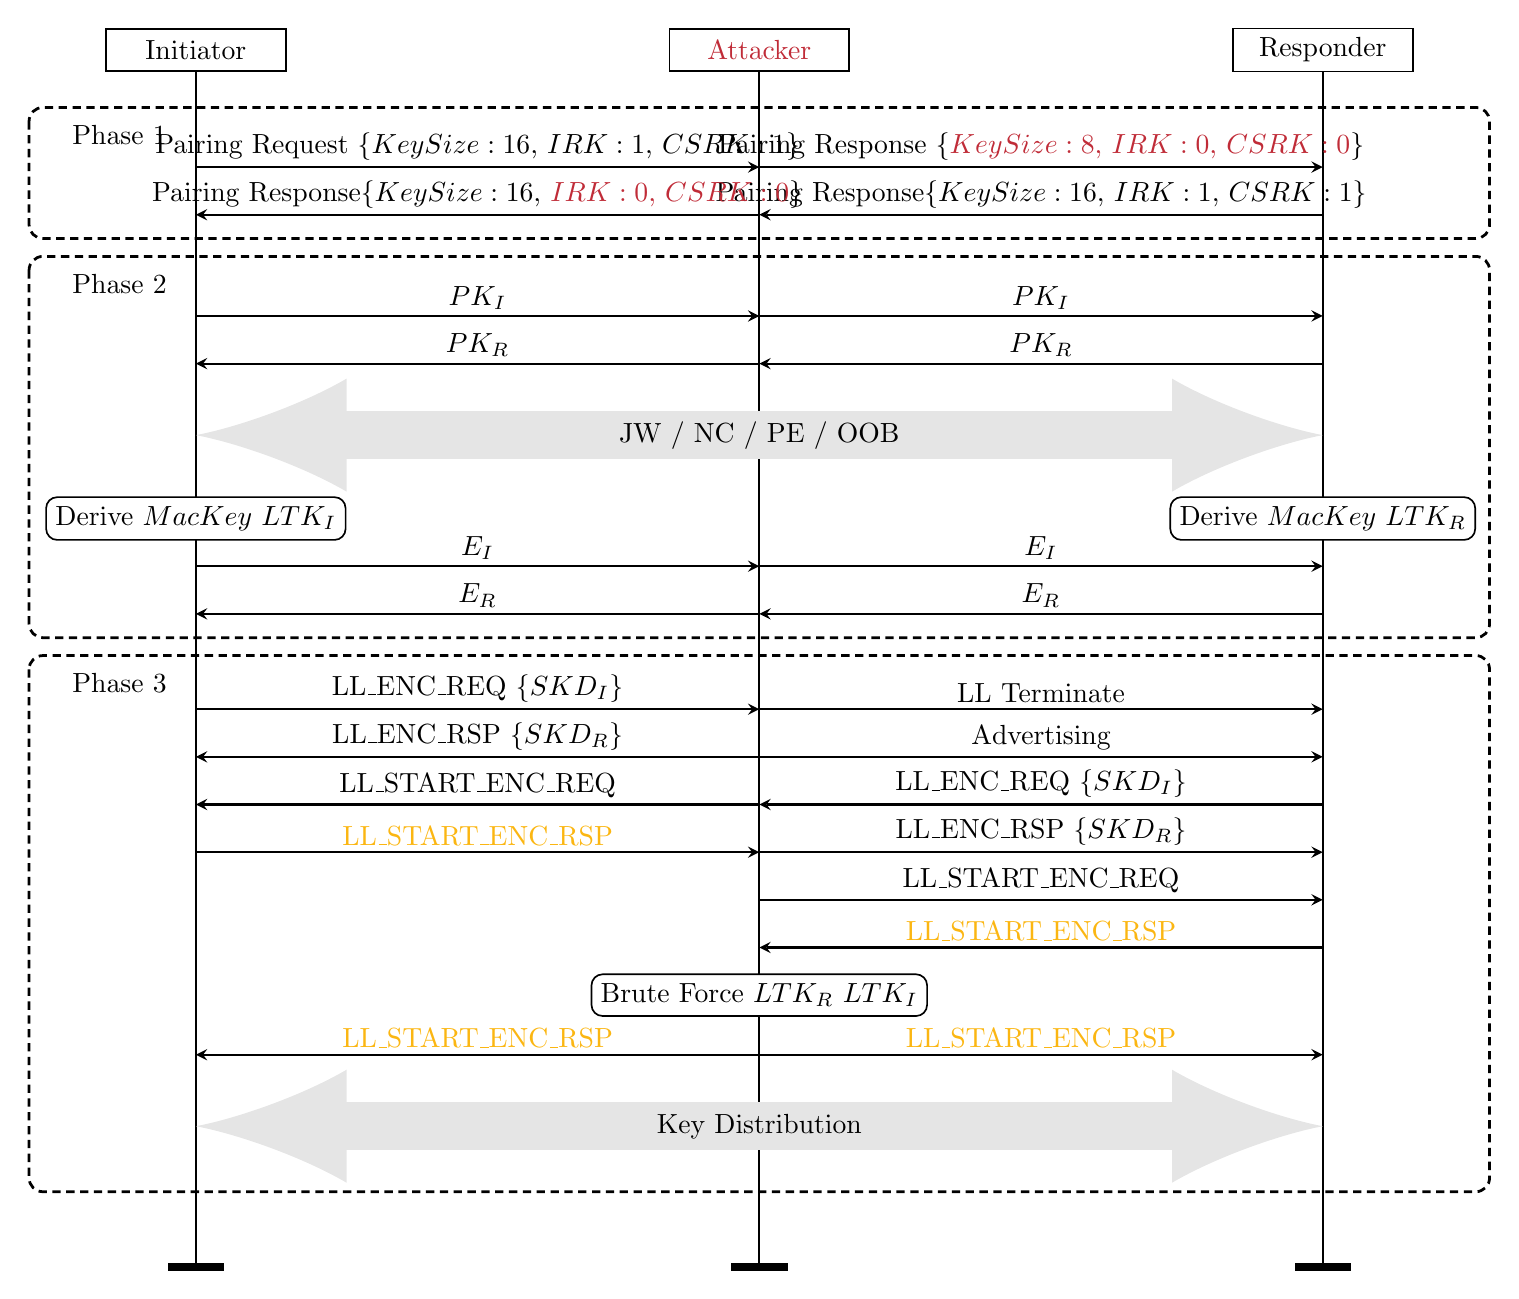
\begin{tikzpicture}

\node[AGENT] (n_initiator) {Initiator};
\node[AGENT, right=0.4\textwidth of n_initiator, text=GaoliangRed] (n_attacker) {Attacker};
\node[AGENT, right=0.4\textwidth of n_attacker] (n_responder) {Responder};
\coordinate (end1) at ($(n_initiator.south)+(0,-100ex)$);
\coordinate (end2) at ($(end1-|n_attacker)$);
\coordinate (end3) at ($(end2-|n_responder)$);
\draw[semithick] (n_initiator.south) -- (end1);
\draw[semithick] (n_attacker.south) -- (end2);
\draw[semithick] (n_responder.south) -- (end3);
\draw[fill=black] ($(end1)+(-1em,0)$) rectangle ($(end1)+(1em,-0.6ex)$);
\draw[fill=black] ($(end2)+(-1em,0)$) rectangle ($(end2)+(1em,-0.6ex)$);
\draw[fill=black] ($(end3)+(-1em,0)$) rectangle ($(end3)+(1em,-0.6ex)$);

% Phase 1: Pairing Feature Exchange
% Downgrade keysize of responder
\coordinate (c_init_req) at ($(n_initiator.south)+(0,-8ex)$);
\coordinate (c_atta_req) at ($(c_init_req-|n_attacker)$);
\coordinate (c_resp_req) at ($(c_init_req-|n_responder)$);
\draw[ARROW] (c_init_req) -- (c_atta_req) node[midway,above=-0.3ex]{Pairing Request \{$KeySize: 16$, $IRK: 1$, $CSRK: 1$\}};
\draw[ARROW] (c_atta_req) -- (c_resp_req) node[midway,above=-0.3ex]{Pairing Response \{\textcolor{GaoliangRed}{$KeySize: 8$, $IRK: 0$, $CSRK: 0$}\}};

\coordinate (c_init_rsp) at ($(c_init_req)+(0,-4ex)$);
\coordinate (c_atta_rsp) at ($(c_init_rsp-|n_attacker)$);
\coordinate (c_resp_rsp) at ($(c_init_rsp-|n_responder)$);
\draw[ARROW] (c_resp_rsp) -- (c_atta_rsp) node[midway,above=-0.3ex]{Pairing Response\{$KeySize: 16$, $IRK: 1$, $CSRK: 1$\}};
\draw[ARROW] (c_atta_rsp) -- (c_init_rsp) node[midway,above=-0.3ex]{Pairing Response\{$KeySize: 16$, \textcolor{GaoliangRed}{$IRK: 0$, $CSRK: 0$}\}};

\coordinate (c_phase1A) at ($(c_init_req)+(-14ex, 5ex)$);
\coordinate (c_phase1B) at ($(c_resp_rsp)+(14ex,-2ex)$);
\draw[BOX] (c_phase1A) rectangle (c_phase1B);
\node[BOXTITLE, below right] at ($(c_phase1A)+(0ex,-0.5ex)$) (n_attacker) {Phase 1};


% Phase 2: Long Term Key (LTK) Generation
\coordinate (c_init_pki) at ($(c_init_rsp)+(0,-8.5ex)$);
\coordinate (c_atta_pki) at ($(c_init_pki-|c_atta_rsp)$);
\coordinate (c_resp_pki) at ($(c_init_pki-|c_resp_rsp)$);
\draw[ARROW] (c_init_pki) -- (c_atta_pki) node[midway,above=-0.3ex]{$PK_I$};
\draw[ARROW] (c_atta_pki) -- (c_resp_pki) node[midway,above=-0.3ex]{$PK_I$};

\coordinate (c_init_pkr) at ($(c_init_pki)+(0,-4ex)$);
\coordinate (c_atta_pkr) at ($(c_init_pkr-|c_atta_pki)$);
\coordinate (c_resp_pkr) at ($(c_init_pkr-|c_resp_pki)$);
\draw[ARROW] (c_resp_pkr) -- (c_atta_pkr) node[midway,above=-0.3ex]{$PK_R$};
\draw[ARROW] (c_atta_pkr) -- (c_init_pkr) node[midway,above=-0.3ex]{$PK_R$};

\coordinate (c_init_user) at ($(c_init_pkr)+(0,-6ex)$);
\coordinate (c_resp_user) at ($(c_init_user-|c_resp_pkr)$);
\draw[DARROW] (c_init_user) to node[black,sloped]{JW / NC / PE / OOB} (c_resp_user);

\coordinate (c_init_derive) at ($(c_init_user)+(0,-7ex)$);
\node[ACTION,minimum height=3.5ex] (n_init_derive) at (c_init_derive) {Derive $MacKey$ $LTK_I$};
\coordinate (c_resp_derive) at ($(c_init_derive-|c_resp_pkr)$);
\node[ACTION,minimum height=3.5ex] (n_resp_derive) at (c_resp_derive) {Derive $MacKey$ $LTK_R$};


\coordinate (c_init_checki) at ($(c_init_derive)+(0,-4ex)$);
\coordinate (c_atta_checki) at ($(c_init_checki-|c_atta_rsp)$);
\coordinate (c_resp_checki) at ($(c_init_checki-|c_resp_rsp)$);
\draw[ARROW] (c_init_checki) -- (c_atta_checki) node[midway,above=-0.3ex]{$E_I$};
\draw[ARROW] (c_atta_checki) -- (c_resp_checki) node[midway,above=-0.3ex]{$E_I$};

\coordinate (c_init_checkr) at ($(c_init_checki)+(0,-4ex)$);
\coordinate (c_atta_checkr) at ($(c_init_checkr-|c_atta_checki)$);
\coordinate (c_resp_checkr) at ($(c_init_checkr-|c_resp_checki)$);
\draw[ARROW] (c_resp_checkr) -- (c_atta_checkr) node[midway,above=-0.3ex]{$E_R$};
\draw[ARROW] (c_atta_checkr) -- (c_init_checkr) node[midway,above=-0.3ex]{$E_R$};

\coordinate (c_phase2A) at ($(c_init_pki)+(-14ex, 5ex)$);
\coordinate (c_phase2B) at ($(c_resp_checkr)+(14ex,-2ex)$);
\draw[BOX] (c_phase2A) rectangle (c_phase2B);
\node[BOXTITLE, below right] at ($(c_phase2A)+(0ex,-0.5ex)$) (n_attacker) {Phase 2};

% Phase 3: Transport Specific Key Distribution
\coordinate (c_init_encreq) at ($(c_init_checkr)+(0,-8ex)$);
\coordinate (c_attai_encreq) at ($(c_init_encreq-|c_atta_checkr)$);
\draw[ARROW] (c_init_encreq) -- (c_attai_encreq) node[midway,above=-0.3ex]{LL\_ENC\_REQ \{$SKD_I$\}};

\coordinate (c_init_encrsp) at ($(c_init_encreq)+(0,-4ex)$);
\coordinate (c_attai_encrsp) at ($(c_init_encrsp-|c_atta_checkr)$);
\draw[ARROW] (c_attai_encrsp) -- (c_init_encrsp) node[midway,above=-0.3ex]{LL\_ENC\_RSP \{$SKD_R$\}};

\coordinate (c_init_startencreq) at ($(c_init_encrsp)+(0,-4ex)$);
\coordinate (c_attai_startencreq) at ($(c_init_startencreq-|c_attai_encrsp)$);
\draw[ARROW] (c_attai_startencreq) -- (c_init_startencreq) node[midway,above=-0.3ex]{LL\_START\_ENC\_REQ};

\coordinate (c_init_startencrsp) at ($(c_init_startencreq)+(0,-4ex)$);
\coordinate (c_attai_startencrsp) at ($(c_init_startencrsp-|c_attai_encrsp)$);
\draw[ARROW] (c_init_startencrsp) -- (c_attai_startencrsp) node[midway,above=-0.3ex]{\textcolor{JidanYellow}{LL\_START\_ENC\_RSP}}; 

\coordinate (c_resp_term) at ($(c_init_encreq-|c_resp_checkr)$);
\draw[ARROW] (c_attai_encreq) -- (c_resp_term) node[midway,above=-0.3ex]{LL Terminate};

\coordinate (c_attar_adv) at ($(c_attai_encreq)+(0,-4ex)$);
\coordinate (c_resp_adv) at ($(c_attar_adv-|c_resp_term)$);
\draw[ARROW] (c_attar_adv) -- (c_resp_adv) node[midway,above=-0.3ex]{Advertising};

\coordinate (c_attar_encreq) at ($(c_attar_adv)+(0,-4ex)$);
\coordinate (c_resp_encreq) at ($(c_attar_encreq-|c_resp_adv)$);
\draw[ARROW] (c_resp_encreq) -- (c_attar_encreq) node[midway,above=-0.3ex]{LL\_ENC\_REQ \{$SKD_I$\}};

\coordinate (c_attar_encrsp) at ($(c_attar_encreq)+(0,-4ex)$);
\coordinate (c_resp_encrsp) at ($(c_attar_encrsp-|c_resp_encreq)$);
\draw[ARROW] (c_attar_encrsp) -- (c_resp_encrsp) node[midway,above=-0.3ex]{LL\_ENC\_RSP \{$SKD_R$\}};

\coordinate (c_attar_startencreq) at ($(c_attar_encrsp)+(0,-4ex)$);
\coordinate (c_resp_startencreq) at ($(c_attar_startencreq-|c_resp_encrsp)$);
\draw[ARROW] (c_attar_startencreq) -- (c_resp_startencreq) node[midway,above=-0.3ex]{LL\_START\_ENC\_REQ};

\coordinate (c_attar_startencrsp) at ($(c_attar_startencreq)+(0,-4ex)$);
\coordinate (c_resp_startencreq) at ($(c_attar_startencrsp-|c_resp_encrsp)$);
\draw[ARROW] (c_resp_startencreq) -- (c_attar_startencrsp) node[midway,above=-0.3ex]{\textcolor{JidanYellow}{LL\_START\_ENC\_RSP}};

\coordinate (c_atta_bf) at ($(c_attar_startencrsp)+(0,-4ex)$);
\node[ACTION,minimum height=3.5ex] (n_atta_bf) at (c_atta_bf) {Brute Force $LTK_R$ $LTK_I$};

\coordinate (c_atta_startencrsp3) at ($(c_atta_bf)+(0,-5ex)$);
\coordinate (c_init_startencrsp3) at ($(c_atta_startencrsp3-|c_init_startencreq)$);
\coordinate (c_resp_startencreq3) at ($(c_atta_startencrsp3-|c_resp_startencreq)$);
\draw[ARROW] (c_atta_startencrsp3) -- (c_init_startencrsp3) node[midway,above=-0.3ex]{\textcolor{JidanYellow}{LL\_START\_ENC\_RSP}};
\draw[ARROW] (c_atta_startencrsp3) -- (c_resp_startencreq3) node[midway,above=-0.3ex]{\textcolor{JidanYellow}{LL\_START\_ENC\_RSP}};

\coordinate (c_init_distribute) at ($(c_init_startencrsp3)+(0,-6ex)$);
\coordinate (c_resp_distribute) at ($(c_init_distribute-|c_resp_startencreq3)$);
\draw[DARROW] (c_init_distribute) to node[black,sloped]{Key Distribution} (c_resp_distribute);

\coordinate (c_phase3A) at ($(c_init_encreq)+(-14ex, 4.5ex)$);
\coordinate (c_phase3B) at ($(c_resp_distribute)+(14ex,-5.5ex)$);
\draw[BOX] (c_phase3A) rectangle (c_phase3B);
\node[BOXTITLE, below right] at ($(c_phase3A)+(0ex,-0.5ex)$) (n_attacker) {Phase 3};


\end{tikzpicture}

\end{document}
